\documentclass[aspectratio=169,12pt,usenames,dvipsnames]{beamer}
\usetheme{Talentsprint}
\usepackage[utf8]{inputenc}
\usepackage{graphics}
\usepackage{ragged2e}
\usepackage{amsfonts}
\usepackage{xcolor}
\usepackage{mathtools}
\usepackage{tcolorbox}
\usepackage{setspace}
\usepackage{lmodern}
\definecolor{swe}{rgb}{0.19, 0.73, 0.56}
\definecolor{lgreen}{RGB}{190,200,198}
\title[FastAPI]{FastAPI}

\begin{document}

{\1
\begin{frame} \vspace{35pt}
	\title[FastAPI]{FastAPI}
	\subtitle{Python Framework}
	\maketitle
\end{frame}
}

\begin{frame}[t]{FastAPI}
\begin{itemize}
  \item Any machine learning model's end goal is a deployment for production purposes.

  \item Building a \href{https://analyticsindiamag.com/the-pricing-plans-for-openais-api-is-out-it-is-not-cheap/}{REST API}(Application Programming Interface) is the best possible way to evaluate model performance.

  \item In python, Django and more evidently \href{https://analyticsindiamag.com/hands-on-guide-to-machine-learning-model-deployment-using-flask/}{Flask} frameworks are used for this purpose.

  \item For machine learning, Flask is preferred more than Django.

  \item Here comes FastAPI which is faster than Flask, providing higher performance boost, easier to code, comes with automatic documentation, provides data validation on input data provided to the server, and many more such features.

\end{itemize}
\end{frame}



\begin{frame}[t]{FastAPI}
\begin{itemize}
\item FastAPI can handle 9000 requests at a time. FastAPI can manage database sessions, web sockets, easy GraphQL injection and many more are still being built.
\item FastAPI is being used by tech giants such as Netflix, Facebook, Microsoft, Uber.
\item Making production-ready RestAPIs with few lines of code is apprehensive.
\end{itemize}
\end{frame}



\begin{frame}[t]{Software Dependencies that are required for FastAPI:-}
\begin{itemize}
\item FastAPI is built upon two major python libraries - Starlette(for web handling) and Pydantic(for data handling).\\
\item Python 3.6+
\item FastAPI
\item ASGI server for production such as Uvicorn or Hypercorn.
\item Pydantic
\end{itemize}
\end{frame}


\begin{frame}[t]{How to install FastAPI?}
\begin{block}{We can install FastAPI using pip}
\begin{itemize}
\item pip install fastapi
\item pip install uvicorn
\end{itemize}
\end{block}
\end{frame}


\begin{frame}[t]{Basic Hello World}
\centering
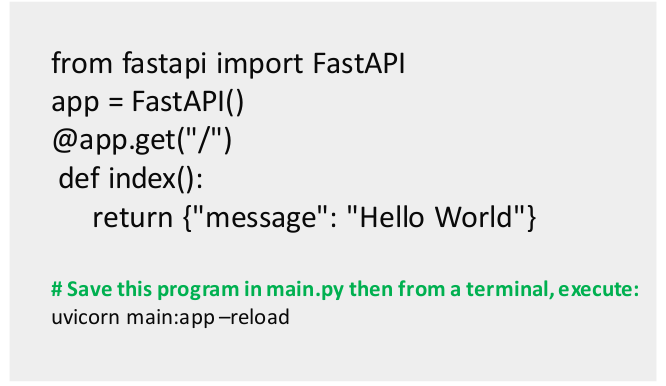
\includegraphics[width=11cm]{FastAPI_Images/AIML_FastAPI_IMG1.png}
\end{frame}


\begin{frame}[t]{Basic Hello World}
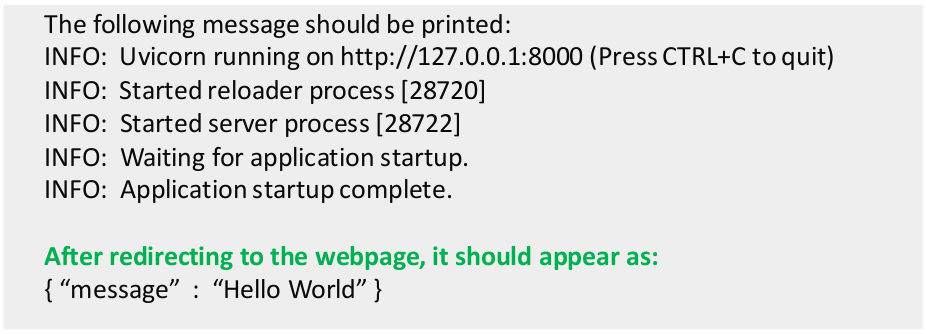
\includegraphics[width=11cm]{FastAPI_Images/AIML_FastAPI_IMG2.png}\\
\small Interactive Documentation {http://127.0.0.1.8000/docs} will show the interactive documentation by Swagger UI.
\end{frame}



\begin{frame}[t]{YAML}
\begin{itemize}
\item YAML is a data serialization format designed for human readability and interaction with scripting languages.
\item PyYAML is a YAML parser and emitter for Python.
\item PyYAML features a complete YAML parser, Unicode support, pickle support, capable extension API, and sensible error messages.
\item PyYAML supports standard YAML tags and provides Pythonspecific tags that allow to represent an arbitrary Python object.
\end{itemize}
\end{frame}


\begin{frame}[t]{Swagger UI}
\begin{itemize}
\item \href{https://swagger.io/tools/swagger-ui/}{Swagger UI} allows anyone - be it your development team or your end consumers - to visualize and interact with the API's resources without having any of the implementation logic in place.
\item It's automatically generated from your OpenAPI (formerly known as Swagger) Specification, with the visual documentation making it easy for back end implementation and client side consumption.
\end{itemize}
\end{frame}


\begin{frame}[t]{Image classification API}
\begin{itemize}
  \item Data annotation (with Unsplash API + Labelme )

  \item Model Training (With Tensorflow)

  \item Making the API (With Uvicorn and FastApi)

  \item Deploying the API on a remote server (With Docker and Google Cloud Platform)

  \item In this project we will try to classify an input image into four classes:

  - City

  - Beach

  - Sunset

  - Trees/Forest

\end{itemize}
\end{frame}


\begin{frame}[t]{MODEL}
\begin{itemize}
  \item We build a classifier using Tensorflow. We will use MobileNet\_V2 as the backbone of the classifier since it is fast and less likely to over-fit given the tiny amount of labeled samples we have, you can easily use it by importing it from keras\_applications.\\
\end{itemize}
\centering
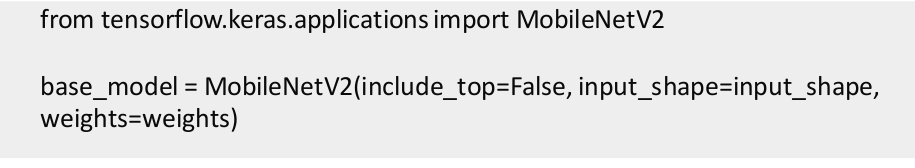
\includegraphics[width=11cm]{FastAPI_Images/AIML_FastAPI_IMG3.png}
\end{frame}


\begin{frame}[t]{Transfer learning}
\begin{itemize}
  \item Commonly used idea is to tackle the lack of labeled samples is to use transfer learning.

  \item It is when you transfer some of the weights learned from a source task (like image classification with a different set of labels) to your target task as the starting point of your training.

   \item This allows for a better initialization compared to starting from random and allows for reusing some of the representations learned on the source task for our multilabel classification.\break

   \centering
   \small {base\_model = MobileNetV2(include\_stop=False, input\_shape=input\_shape, weights="imagenet")}

\end{itemize}
\end{frame}



\begin{frame}[t]{Training}
\begin{itemize}
  \item We split the dataset into two folds, training and validation and use the binary\_crossentropy as our target along with the binary\_accuracy as the evaluation metric.
\end{itemize}
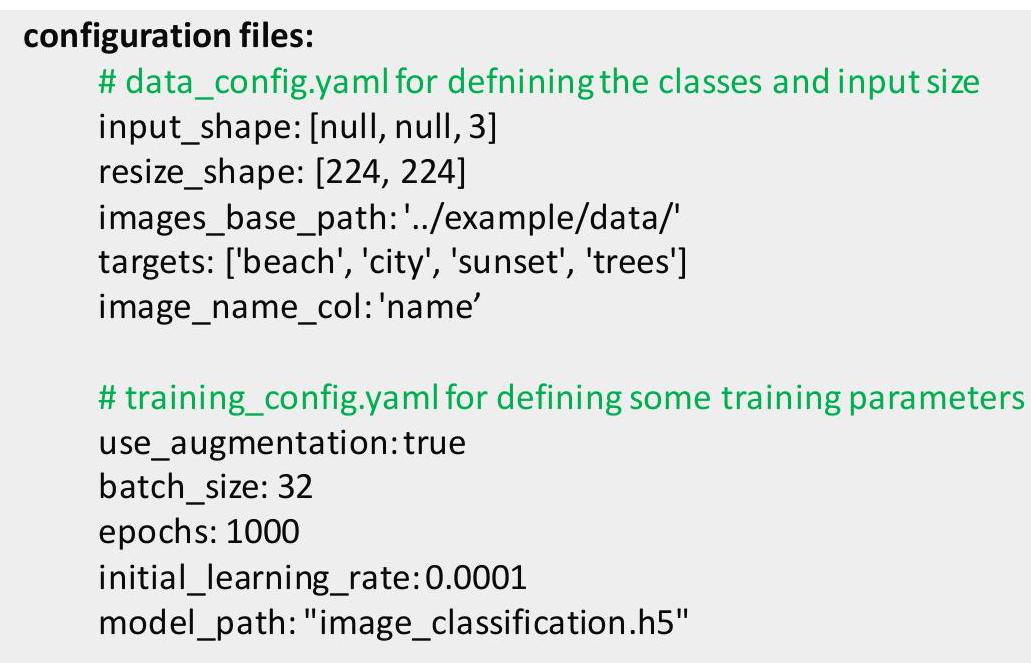
\includegraphics[width=7cm]{FastAPI_Images/AIML_FastAPI_IMG4.png}
\end{frame}


\begin{frame}[t]{Making the API}
\begin{itemize}
\item We will be using FastAPI to expose a predictor through an easy to use API that can take as input an image file and outputs a JSON with the classification scores for each class.

\item Predictor class that can easily load a tensorflow.keras model and have a method to classify an image that is in the form of a file object.
\end{itemize}
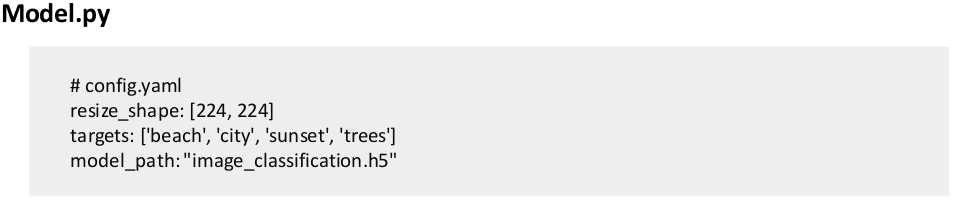
\includegraphics[width=9cm]{FastAPI_Images/AIML_FastAPI_IMG5.png}
\end{frame}


\begin{frame}[t]{The main file of our API becomes trivial when using FastAPI:}
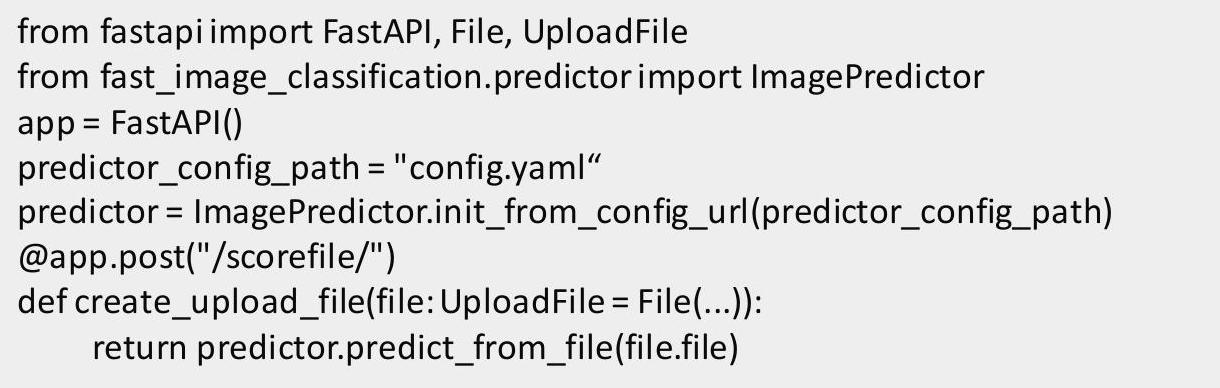
\includegraphics[width=11cm]{FastAPI_Images/AIML_FastAPI_IMG6.png}
\end{frame}

{ \1
\begin{frame}
	\title{Thanks!!}
	\subtitle{Questions?}
	\maketitle
\end{frame}
}

\end{document}
